\documentclass[a4paper,12pt]{article}

%\usepackage[pdftex]{graphicx}
\usepackage{amsmath}
%\usepackage[latin1]{inputenc}
%\usepackage{hyperref}
%\usepackage[T1]{fontenc}
%\usepackage[utf8]{inputenc}
%%GD Quand je mets usepackage[utf8]{inputenc} je n'arrive plus à compiler la biblio
%J'ai essayé de débuger : je n'y suis pas arrivé
\usepackage{rotating}
\usepackage{setspace}
\usepackage{lscape}
\usepackage[round]{natbib}
\usepackage{multirow}
\usepackage{rotating}
\usepackage{vmargin}
\usepackage{epstopdf}
\usepackage{hyperref}
\usepackage{float}
\usepackage{caption}
\usepackage[tableposition=top]{caption}
\usepackage{amsfonts}
\usepackage{bbold}
\usepackage{bbm}
\usepackage[flushleft]{threeparttable}
%\usepackage{bbold}
%\usepackage[T1]{fontenc}
% JH : impossible de compiler avec le package bbold, remplacé par amsfonts
% LP : impossible de compiler avec le package bbold, remplacé par bbm
\usepackage{upgreek}
\usepackage{comment}
\includecomment{commentGD}
\usepackage[draft]{todonotes}
%\usepackage[disable]{todonotes}
%%GDPour cacher les notes, \usepackage[disable]{todonotes}

\usepackage{setspace}

%\usepackage[nolists, figuresfirst]{endfloat}
%\usepackage{sidefloat}

\setlength{\abovecaptionskip}{-8pt}

%\usepackage[usenames]{color}
%\definecolor{grey}{rgb}{0.35,0.35,0.35}
%\definecolor{webdarkblue}{rgb}{0,0,0.4}
%\definecolor{orange}{rgb}{0.7,0.2,0.05}


%\usepackage[pdfcreator={PDFLaTeX}, pdfproducer={PDFLaTeX}, pdfstartview=FitH, pdfpagemode=UseOutlines, pagebackref=false, colorlinks={true},
%citecolor={webdarkblue}, linkcolor={webdarkblue},
%urlcolor={webdarkblue}]{hyperref}



%\addtolength{\oddsidemargin}{-0.4in}
%\addtolength{\evensidemargin}{-0.4in}
%\addtolength{\textwidth}{0.8in} \addtolength{\topmargin}{-0.85in}
%\addtolength{\textheight}{1.7in}
\renewcommand{\baselinestretch}{1.2}

\newcommand\cites[1]{\citeauthor{#1}'s\ (\citeyear{#1})}

\newcommand\citeh[1]{\citeauthor{#1}'\ (\citeyear{#1})}

\setmarginsrb{3cm}{2cm}{3cm}{2cm}{0,5cm}{0,5cm}{0,3cm}{0,5cm}



% commands

\newcommand{\bi}{\begin{itemize}}
\newcommand{\ei}{\end{itemize}}
\newcommand{\be}{\begin{enumerate}}
\newcommand{\ee}{\end{enumerate}}
\newcommand{\bd}{\begin{description}}
\newcommand{\ed}{\end{description}}
\newcommand{\beqa}{\begin{eqnarray}}
\newcommand{\eeqa}{\end{eqnarray}}
\newcommand{\beq}{\begin{equation}}
\newcommand{\eeq}{\end{equation}}
\newcommand{\bs}{\bigskip}
\newcommand{\A}{$^a$}
\newcommand{\B}{$^b$}
\newcommand{\C}{$^c$}

\renewcommand{\baselinestretch}{1.2}
%\doublespacing

%\linespread{1.6}

%\newcommand{\note}[1]{\footnote{\begin{doublespace}#1\end{doublespace}}}


\begin{document}


\title{\textsc{International Transport costs:\\New Findings from modeling additive costs} \\
Answer to Referee 1}

\author{Guillaume \textsc{Daudin}\thanks{%
Université Paris-Dauphine, PSL University, CNRS, 8007, IRD, 260, LEDa, DIAL, 75016, Paris, France ; email: \url{guillaume.daudin@dauphine.psl.eu}}  \qquad J\'{e}r\^{o}me \textsc{H\'{e}ricourt} \thanks{Universit\'{e} de Lille - LEM-CNRS UMR 9221, France \& CEPII, France; email: \url{jerome.hericourt@univ-lille.fr}}\qquad Lise \textsc{Patureau}\thanks{Corresponding author.
University Paris-Dauphine \& PSL University, LEDa, 75016 Paris, France;  email: \url{lise.patureau@dauphine.psl.eu} } }


\date{September 2021}
 \maketitle
\bigskip

We would like to thank you for your insightful comments. They led us to introduce some
significant changes to the paper that we hope address your concerns. We first give you an overview
of the revision (Section\ref{sec:main_changes}) before answering in detail each of your comments (Section\ref{sec:detailed_answers}). Number of sections, pages and equations mentioned in the text refer to the revised version.

\section{Main changes \label{sec:main_changes}}


\begin{itemize}
%\item Based on your comment 1.2 (\textit{The aggregation problem}), we have investigated the case with $s=3$ and $k=10$ for the industry/product aggregation levels respectively. Our initial choice of retaining $s=3$ at the sectoral level, $k=5$ at the product level was driven by the use of Hummel's dataset available over 1974-2004 with $k=5$ the finest degree of aggregation. In the submitted version, we used the original Hummel's database (available on his webpage from 1974 to 2003, which we completed by the US Bureau of census import database over the period 2005-2013. In Hummels' (2007) database, which we use until 2004, the finest degree of classification is at the 5-degree level until 2004. For comparability reasons over time, we have adopted the same degree of classification $k=5$ for the following years (based on the original Census dataset). As a result, in the submitted version, transport costs are estimated at the 3-digit sector level as benchmark estimate, exploiting product heterogeneity at the 5-digit level (for a given origin country, and conditional on year and transport mode).
%
%    Switching to $k=10$ as benchmark disaggregation level for the product dimension would require resorting on US Census dataset only. It is true that the original annual Census data reports trade at the origin country-HS 10 product-district level of aggregation. However, the Census bureau can provide data disaggregated at the $k=10$ product level only starting in 1989. Some of these data are in physical storage and were not accessible because of the Covid-19 pandemic (1989-1996, but also 2000 and 2001). In september 2021, they are still not accessible. Waiting for them contributed to making this revision quite late. This deprives us from the very first years 1974-1996 and 2000-2001. For this period, we can only resort on Hummel's dataset, with $k=5$ the finest product level category. This is a non-negligible cost as we are interested in the long-term evolution of trade costs.
%
%    As a result, we decided to adopt the following strategy in the revised version. As benchmark, we still consider the 5/3 product/sector classification (as in the submitted version), as this allows us to preserve (as far as possible) the largest time coverage. We check the robustness of our results to the 10/3 classification, for the available years. This is made in Section XXX.
%
%    \textbf{LP: Pas sure que ce point doive etre mis ici, pas main change du coup}
    


\item Based on your comment 1.1 (\textit{The endogeneity problem}), the benchmark regression (non-linear least squares) is now completed by a two-stage procedure, where the fas price is instrumented by tax duties and its own lag - see section 4.3 and appendix B.4 in the paper, and section 2.1.2 of this letter.

\item Based on your main comment 1, the paper has been rewritten so as to be more in line with Hummel's (2004) methodology. Specifically, we now start from the elasticity of total transport costs to the unit price $\beta$, which we show also corresponds to the share of additive costs. From this, we can deduce the additive / ad-valorem components ($t,\tau$) rather than the other way round (as in the submitted version). We thank the referee for pointing this out, as this contributes to a more straightforward and intuitive understanding of our estimation method.

\item What about the big picture?
\end{itemize}

We now answer in detail each of your comments given in italics.

\section{Detailed answers \label{sec:detailed_answers}}


\subsection{Critique 1: Empirical Strategy}

\textit{Using the notation of the authors, they are intreated
in identifying the share of the specific cost in the total transport cost. Namely,}
\begin{eqnarray*}
&& \frac{\frac{t_{is(k)}}{\tilde{p}_{ik}}}{\tau_{is(k)}-1 + \frac{t_{is(k)}}{\tilde{p}_{is(k)}}} \\
\text{or,} &&\frac{t_{is(k)}}{(\tau_{is(k)}-1)\tilde{p}_{is(k)} + t_{is(k)}}
\end{eqnarray*}

\textit{The way they approach the problem is that they assume that (a) $\tau_{ik} = \tau_i\tau_{k}$,
(b) $t_{ik} = t_i +t_k$, and (c) $t_k$ and $\tau_k$ are uniform across products within industry
s. After imposing these assumptions, they estimate the following specification}

\begin{equation}
\ln\left(\frac{p_{ik}}{\widetilde{p}_{ik}}-1 \right)= \ln \left(\tau_{i} \times \tau_{s(k)} -1+\frac{t_{i} + t_{s(k)}}{\widetilde{p}_{ik}} \right) + \epsilon_{ik} \label{eq:equation0}
\end{equation}

\textit{in which $\tau_i$, $\tau_{s(k)}$, $t_i$, and $t_{s(k)}$ are identified as fixed effects coefficients.
In my opinion this choice of strategy is quite sub-optimal, as (i) it relies on
the strong assumptions highlighted above, (ii) it is computationally expensive
as noted by the authors on multiple occasions, and (iii) it is subject to an
endogeneity problem, which the authors disregard with one sentence, but which
is rather detrimental in my opinion.}

\textbf{Our answer:}\\

%\paragraph{Strategy of answer} To clarify the discussion, we decided to answer concerns (i) and (iii) each in turn. As regards to point (ii), we run the referee's proposed estimation method without relying on instrumental variables; this way, the results are comparable with the benchmark results, the only change being the estimation strategy (Section \ref{subsec:functional_form} of the letter). As noted above, this drove us to maintain our estimation method as benchmark. As regards to point (iii), we instrument fas prices at the $k=$ 10-digit level, still based on our original estimation strategy (but switching to a finest product category disaggregation level $k=10$). This allows a direct comparison of the results obtained in the non-linear least squares regression with those obtained with IV (with $s=3$ digit at the sector level and $k=10$ at the product level in both cases). This is developed in \textbf{Section ??? of the letter}.


The three points raised by the referee indeed deserve careful consideration. We provide separate answers to each of them below, starting with points (i) and (iii), and finishing with point (ii).

\subsubsection{On the justifications for our empirical approach}

\paragraph{About the key assumption of separability}
Our main empirical equation and its underlying assumptions regarding the separability of transport costs between their country- and product-level components draw on the one proposed by \citet{Irrazabal_2015} to estimate the share of additive costs in a firm-level context. It relies on a simple theoretical framework with minimal assumptions, and is compatible with most approaches within the so-called category of ``New Trade Theories''.

Further, we provide a robustness check for this separative assumption, in Section 4.1 of the paper (\textbf{Table 2, previously submitted version and revised version XXX CHECK AT THE END XXX}). We check the robustness of our results by re-running the estimation without the separability assumption. This comes at the cost of a substantial increase in the number of fixed effects to include in the regression. Based on the numbers of countries and sectors reported in \textbf{Table 1 of the submitted version and revised version  XXX CHECK AT THE ENDXXX} (188 countries, 230 3-digit sectors), it would mean including 86,480 fixed effects ($188\times230\times2$ for the two additive and multiplicative costs) rather than ``only'' 836 ($(188+230)\times 2$). This is computationally not tractable. For this reason, we have decided to run the robustness check on a reduced sample. If it is smaller in terms of observations (2,381 for Air, 2,798 for Vessel on average over the period 1974-2013 XXX 2019 ??? XXX, vs around 29,000 on the complete sample, see Table 1), it yet remains quite large in terms of trade coverage, as the selected countries and sectors (at the 3-digit level) constitute 80\% of the total value of flows (on a yearly basis). As we conclude at the end of Section 4.1, whatever the transport mode and for both types of transport costs, the trend patterns of international transport costs are very similar whether estimated under the separability assumption or not - see in particular Figures 6 and 7 on pp. 25-26. Given that the restricted sample covers 80\% of the total trade flows of the US economy, we hope to convince you that this result can be extended to the whole dataset.


\paragraph{On the use of non-linear least squares (NLS)}

The referee writes \textit{A more natural approach is what the authors, at some point, refer to as the Hummel's Methodology. That is, one can alternatively estimate the share of the additive component as:}

$$\frac{t_{ik}}{ (\tau_{ik}-1)\tilde{p}_{ik} + t_{ik}} = \beta_{ik}$$

\textit{where $\beta_{ik}$ is the elasticity of transport costs w.r.t. unit price} in absolute value, as shown with more details in Appendix \ref{app:interpret_beta} through Equation (\ref{eq:Hummels}). \textit{Given the authors' objective and the data they are using, $\beta$ can be separately estimated
for each industry-country pair using the following regression:}

\begin{equation}
\ln f_{ikd} = \beta_{is(k)}\ln \tilde{p}_{ikd} + \text{Controls}_{ikd} +\epsilon_{ikd} \label{eq:estimation_ref1}
\end{equation}

\textit{where $d$ denotes the US district of entry and $k$ denotes an HS10 product} ($f_{ikd}$ being the transport costs). \textit{The
identification of $\beta_{ik}$, in this case, would rely on the across HS10 product and
district-of-entry variation in $f_{ik}$ and $p_{ik}$. Estimating the above equation would
obviously require that the authors do not aggregate up the raw Census data
across all districts and all 10-digit products pertaining to the same 5-digit category.}

\textbf{Our answer:}
As highlighted by the referee, our estimated equation requires non-linear estimation methods, such as Non-Linear Least Squares. However, even with another formulation, such as the one suggested by the referee in Equation (\ref{eq:estimation_ref1}), we would still be constrained to resort to non-linear estimators. This is due to the necessity of imposing an \textit{ex-ante} restriction on parameters, i.e. $\tau \geq 1$ and $t \geq 0$, or $0 \leq  \beta \leq 1$. Should we relax these restrictions, standard linear, least squares estimates often deliver negative, meaningless estimates. In this respect, implementing the referee's method (see below) does not suppress the requirement of resorting on non-linear estimates (and the computational, time-consuming burden it induces). Imposing this parameters constraint was not made clear enough in the initial version, and we did our best to make this very important justification clearer in the revised version - see footnote 16XXX page 8: ``One may object that we could preserve the estimation at the 5-digit level by running an OLS estimation on the equation taken in level, i.e.`on the basis of Equation (\ref{eq:base_estimee}), specifying the error term additively. This would not solve the problem though, for three main complementary reasons.
First, at the 5-digit level the number of fixed effects to include in the estimation would be more than 430,000 (with 216 countries and 2,029 products), making the estimation computationally extremely burdensome, even in OLS.
Imposing Equations (\ref{eq:ad-valorem}) and (\ref{eq:add}) to reduce the number of fixed effects would drive us back to the non-linearity issue for fixed effects.
Second, making the error term (specified as following a normal law centered on 0) enter Equation (\ref{eq:base_estimee}) additively implies negative values for some of the estimated residuals $\widehat{\epsilon}_{ik}$, which is inconsistent with the constraint that $\frac{p_{ik}}{\widetilde{p}_{ik}}>1$.
Third, estimating the equation in level does not eliminate the fact that it is non-linear by nature, as long as there are additive costs to estimate (see Equation (\ref{eq:base_estimee}) for $t_{ik} \neq 0$)''


Of course, this does not prevent us for taking full account of your suggestion to adopt an alternative estimation method (summarized in Equation (\ref{eq:estimation_ref1}). It turns out that this method does not go without a few important limitations, that justify maintaining our initial estimation strategy as the baseline in the building block of the paper.\textbf{The referee's method is presented in the online appendix XXX WHERE??? XXX, and we refer to it in Footnote XXX of the paper}. We develop the analysis we held below.



\paragraph{Exploring Referee's alternative functional form \label{subsec:functional_form}}

The estimation strategy suggested by the referee starts from Equation (\ref{eq:Hummels}) linking transport costs and unit prices as assumed in Hummels (2007). As shown in Subsection (\ref{ssec:interpret_beta}), the elasticity of transport costs to unit prices $\beta_{ik}$ (in absolute value) also corresponds to the share of additive costs in total transport costs. The share of additive costs can hence be uncovered by regressing transport costs on unit (ie, fas) prices. Specifically, the referee suggests to run the estimation based on Equation (\ref{eq:estimation_ref1}).

Precisely, by year and transport mode, this implies running the estimation for each country of origin $i$ and each sector $s(k)$ = 3 digit sector, exploiting the variability between sub-sectors at the 10-digit level ($k$) and between ports of entry in the US ($d$). We have implemented the referee's method over the years for which we already have the data, i.e. the years 2005-2013 (already used in the submitted version).

Notice that we are aware of the referee's suggestion to run his/her estimation strategy considering sectoral aggregation at the 5-digit level (with $k=10$). We yet keep considering sectors at the 3-digit aggregation level, in view of being able to compare the pros and cons of the referee's method versus ours, including those years for which the finest disaggregation level is $k=5$ (i.e., the original Hummel's dataset \textbf{over 1974-1988, as the US Bureau of census import database starts in 1989.})

Despite its interest, implementing the referee's method uncovered some drawbacks, that in our view, outweighs those of our method (in particular associated with \textit{Assumptions (a) $\tau_{ik} = \tau_i\tau_{k}$, and (b) $t_{ik} = t_i+ t_{k}$.}) We develop our results and conclusion by answering each argument made by the referee at a time.

Our answer can be articulated in two steps. First, we challenge the advantages that the referee's estimation method would bring in comparison with our's. Second, we emphasize the drawbacks induced by this method. XXX HERE XXX

%
%\paragraph{What we do}
%
%Our estimated equation is written as Equation (\ref{eq:equation0}) with $s$= 3 (or 4) digit and $k$=5 digit (based on Hummel's original dataset from 1974-2004). We thus exploit the variability of transport costs between countries and between 3-digit sectors (conditional on a year and a transport mode, air or vessel). To sum up our methodology:
%\begin{itemize}
%\item Estimating Equation \ref{eq:equation0} provides us with estimates of $\hat{t}_i$, $\hat{t}_{s(k)}$, $\hat{\tau}_i$, $\hat{\tau}_{s(k)}$.
%\item We rebuild
%\begin{eqnarray*}
%\hat{t}_{is(k)} &= &\hat{t}_{i}+\hat{t}_{s(k)} \\
%\hat{\tau}_{is(k)} &= & \hat{\tau}_{i}\times\hat{\tau}_{s(k)}
%\end{eqnarray*}
%\item We deduce the weighted average value of each component $\bar{t}$, $\bar{\tau}$ by year and transport mode, the weighting scheme being the relative value of the flows for each $i,s$ flow, as well as the median, the maximum and the minimum values.
%\item With this in hand, we can (among other things) obtain the estimated share of additive costs in total transport costs for each $i,k$ flow:
%
%
%$$\hat{\beta}_{ik} = \frac{\frac{\hat{t}_{is(k)}}{\tilde{p}_{ik}}}{\tau_{is(k)}-1 + \frac{t_{is(k)}}{\tilde{p}_{is(k)}}} $$
%\end{itemize}
%
%\paragraph{What the referee suggests to do}
%
%The estimation strategy suggested by the referee starts from Equation (\ref{eq:Hummels}) linking transport costs and unit prices as assumed in Hummels (2007). As shown in Subsection (\ref{ssec:interpret_beta}), the elasticity of transport costs to unit prices $\beta_{ik}$ (in absolute value) also corresponds to the share of additive costs in total transport costs. The share of additive costs can hence be uncovered by regressing transport costs on unit (ie, fas) prices. Specifically, the referee suggests to run the estimation based on Equation (\ref{eq:estimation_ref1}).
%
%Precisely, by year and transport mode, this implies running the estimation for each country of origin $i$ and each sector $s(k)$ = 3 digit sector, exploiting the variability between sub-sectors at the 10 digit level ($k$) and between ports of entry in the US ($d$).\footnote{The referee suggests to run his/her proposed estimation strategy considering sectoral aggregation at the 5-digit level (with $k=10$). We followed his suggestion but considering the 3-digit level. We made this choice in view of being able to compare the pros and cons of the referee's method versus ours. In Hummels' (2007) database, which we use until 2004, the finest degree of classification is at the 5-degree level until 2004. For comparability reasons over time, we adopt the same degree of classification $k=5$ for the following years (based on the original Census dataset). As a result, transport costs are estimated at the 3-digit level as benchmark estimate, exploiting heterogeneity at the 5-digit level (for a given origin country, and conditional on year and transport mode). This has driven us to retain $s=3$ when implementing the referee's method, in view of preserving comparability between both strategies.}


\paragraph{a) The advantages of the referee's method are not as important as suggested}


\begin{itemize}
\item the referee writes \textit{The first advantage of this so-called Hummel's Approach is that the above
regression can be estimated separately for various country-industry pairs, without
imposing Assumptions (a) $\tau_{ik} = \tau_i\tau_{k}$, and (b) $t_{ik} = t_i+ t_{k}$.} \\

\textbf{Our answer:}

First, the separability assumption does not seem to be a strong assumption. This is based on the conclusion drawn from the robustness check on a reduced sample (in the submitted version, considering $s=3, k=5$, and in the revised version, considering $s=3, k=10$). If it is smaller in terms of observations,\footnote{In the restricted sample, we have around 25 sectors from 14 countries for Air transport, vs 230 sectors from 190 countries in the large sample; and around 50 sectors from 20 countries for Vessel, vs 600 sectors from 190 countries in the complete sample). Given that the reduced sample makes for 80\% of the total value of trade flows, this suggests that the vast majority of US imports comes from a selected range of countries, in a selected range of sectors.} it yet remains quite large in terms of trade coverage, as the selected countries and sectors (at the 3-digit level) constitute 80\% of the total value of flows (on a yearly basis). As we conclude at the end of Section XXX, whatever the transport mode and for both types of transport costs, the trend patterns of international transport costs are very similar whether estimated under the separability assumption or not. Given that the restricted sample covers 80\% of the total trade flows of the US economy, we hope to convince you that this result can be extended to the whole dataset.


Second, the referee's method imposes a drastic selection of countries / sectors to be included in the estimation. Specifically, since the estimation method is run at the sector-origin country level (on top of being year-mode specific), the number of flows within each country-sector pair should be large enough to more than cover the number of $k$- product and $d$- entry port fixed effects. This substantially reduces the number of point estimates, as well as the value of trade flows covered relative to the  benchmark method, as summarized in Table .



\item the referee writes \textit{The second advantage is that there is a handful of previously-proposed instruments (e.g., HS-10 product-specific tariff rates or lagged prices), which the authors can use to overcome the endogeneity problem.} \\

     \textbf{Our answer:}
We thank the referee for this valuable suggestion. It is worth noticing that we can also handle the instrumentation of fas prices at the HS-10 level with our method - which we do in the revised version.


\item the referee writes \textit{The third advantage is that, by adopting this approach, the comparison between the paper [...] and those in Hummels (2007) would become more transparent.}\\
     \textbf{Our answer:}
     We agree with the referee that the comparison with the literature (\citealp{hummels2007}) in particular) was not straightforward for the reader in the submitted version. We did our best to make the comparison clearer in the revised version, yet in a way consistent with our estimation method. In contrast to the submitted version, the paper now starts from the relation linking transport costs to the unit price specified in Hummels (2007):
    \begin{equation}
    f_{ikt} = X_{is(k)t}\widetilde{p}_{ikt}^{-\beta_{ikt}} \label{eq:Hummels}
    \end{equation}

     with $f_{ikt} = \frac{p_{ikt}}{\widetilde{p}_{ikt}} -1 $ the transport costs measure, $p_{ikt}$ ($\widetilde{p}_{ikt}$) the cif (fas) price and $\beta_{ik}$ the price-elasticity of transport costs, which also corresponds to the share of additive costs in total transport costs (as we now show in the paper's appendix):

     \begin{equation}
     \beta_{ikt} = \frac{\frac{t_{is(k)}}{\widetilde{p}_{ikt}}}{\tau_{is(k)}-1+\frac{t_{is(k)}}{\widetilde{p}_{ikt}} } \label{eq:beta_TC}
     \end{equation}

     As underlined in the paper (both submitted and revised versions), Equation (\ref{eq:Hummels}) lies at the root of Hummels's (2007) method, as he estimates Equation (\ref{eq:Hummels}) on a panel basis and at the sectoral $s(k)$ basis, yielding to estimates of $\beta_{is(k)}$ that are invariant over time (but mode-specific).

     Two alternative strategies are yet available. Let us start with the referee's method. It starts from the functional form linking transport costs and the fas price as specified in the Hummels's equation (\ref{eq:Hummels}). Taken in log (on a mode/yearly basis), it is written as:
     $$\ln f_{ikd} = \beta_{is(k)}\ln \widetilde{p}_{ikd} +\text{Controls}_{ikd}+ \varepsilon_{ikd}$$

     From this, one can then recover the levels of additive / multiplicative transports costs. Denoting $\widehat{\beta}_{is(k)}$ the estimated $\beta$ for a given sector-country $i,s(k)$, one can indeed solve the following two-equation system:

\begin{eqnarray}
p_{ik} &=& \tau_{is(k)}\widetilde{p}_{ik} +t_{is(k)} \label{eq:system1}\\
\frac{t_{is(k)}}{(\tau_{is(k)}-1)\widetilde{p}_{ik}+ t_{is(k)}} &=& \widehat{\beta}_{is(k)}  \label{eq:system2}
\end{eqnarray}

\noindent with $p_{ik}$ and $\widetilde{p}_{ik}$ the cif and fas prices observed in our dataset (conditional on a given year-transport mode). With 2 equations and 2 endogenous variables, the system might be solved.

     Alternatively, our method rather starts from the definition of transport costs as:
     $$\ln f_{ik} = \ln\left(\tau_{is(k)} -1 + \frac{t_{is(k)}}{\widetilde{p}_{ik}}\right) +\varepsilon_{ik}$$
from which we deduce the additive/multiplicative costs $\widehat{t}_{is(k)}$, $\widehat{\tau}_{is(k)}$ (on a mode/yearly basis). Then, relying on the Hummels' equation, one can deduce the share of additive costs in total transport costs $\beta_{ik}$ through Equation (\ref{eq:beta_TC}), again on a mode/yearly basis.

In this respect, the two methods are equivalent, in that they both allow to uncover the share of additive costs in total transport costs $\beta$, as well as the value of each trade costs component ($t,\tau$), that vary over time and sectors (and transport mode). Put it differently, our method is consistent with Hummel's methodology - provided that it is adequately reported as such. We agree that this was not sufficiently transparent in the submitted version. We hope that the revised version now fits the referee's expectations on this point.

\end{itemize}



\paragraph{b) The costs are high}
\begin{itemize}
\item[Concern 1] The suggested estimation strategy implies having much less data to exploit, for two reasons.
\begin{enumerate}
\item Information about the port of entry are only available since 1989. Implementing the referee's method would hence necessarily reduce the time coverage of our analysis by 15 years (1974-1988). In our view, the historical coverage is interesting per se, as it provides useful insights about how transport costs have evolved over time. Eliminating this dimension of the paper would be detrimental to its value-added.
\item As underlined before, the method is run country by country, and 3-digit sector by 3-digit sector, exploiting the variability within each country-3d sector across 10-d sub-sectors and ports of entry. Yet, it appears that for many couples (country, 3-digit sector), there is too few variability across sub-sectors or ports en entry given the number of fixed effects included in the regression, such that estimation can not be run. This can be seen comparing the number of observations by year/ transport mode with our method / with the referee's method reported in Table XXX \textbf{TO DO}. Put it differently, this methodology discards countries which export a limited range of goods to the US and/or which arrive in the USA through the same ports of entry. It excludes XXX \% of trade flows and XXX \% of trade in value. In this respect, the induced selection bias reduces the general scope of the transport costs estimates.

    \end{enumerate}
\item[Concern 2] Given that the estimation method is run at the country-sector level (exploiting heterogeneity \textit{within} a given country-sector pair), it implicitly assumes that transport costs are independent \textit{across} sectors and across origin countries. Put it in plain words, it means that transport costs of say, tissues, have nothing in common whether those goods comes from France or from Bangladesh; or that transport costs that apply to imported goods from France have no common component across sectors. In both cases, one might view this as a disputable assumption. By contrast, our method exploits the fact that transport costs have a both a country-specific component and a sector-specific component. \textbf{This stands in line with ...  FAIRE REFERENCE A DES PAPIERS EN TRADE QUI ONT DES TRADE COSTS Pays-spécifique}


\item[Concern 3] The suggested method features less accuracy in the estimation of the $\beta$. If we take the value of the $\beta$ by itself, there is no criteria to discriminate between the value estimated with our method and the one obtained with the suggested method (when, of course, run on the same sample). Things are more clear-cut in terms of accuracy of the estimation. Specifically, our method yields a more precise estimation of the $\beta$ than the referee's method. To develop on this, for each year and transport mode:
    \begin{itemize}
    \item With the referee's method, we estimate one value for the share of additive component $beta$ at the $i,s$ level denoted $\hat{\beta}^{ref}_{is(k)}$ associated with a standard deviation $SD_{is}$, by year and transport mode. From this, we can approximate the 5-95\% threshold values through:
        $$\hat{\beta}_{is}^{min,ref} = \hat{\beta}^{ref}_{is(k)} - 1.96 SD_{is},\quad \hat{\beta}_{is}^{max,ref} = \hat{\beta}^{ref}_{is(k)} + 1.96 SD_{is}$$

        From this, we can deduce the confidence interval $CI^{ref}_{is} = \hat{\beta}_{is}^{max,ref} - \hat{\beta}_{is}^{min,ref}$.

    \item  Our method does not yield an estimate of $\beta_{is}$ and an associated standard deviation, so that we cannot directly compare the precision of the estimation. Rather, our method provides estimates of the underlying trade costs components ($\widehat{\tau}_i$, $\widehat{\tau}_s$, $\widehat{t}_i$, $\widehat{t}_s$) with an associated matrix of variance-covariance, from which we can rebuild $\beta_{is}$. We then deduce the accuracy of the $\beta$ estimate by relying on bootstrap method. Specifically, on a yearly/mode basis we draw a distribution of trade costs components and associated $\beta_{is}$ (10,000 random draws) from which we can compute the mean, the median and the 5-95 threshold values for each couple $i,s$. Noticing $\beta_{is}^{95}$ and $\beta_{is}^{05}$ the associated thresholds, we then obtain the confidence interval $CI_{is}= \beta_{is}^{95}- \beta_{is}^{05}$.\footnote{Notice that this should be made on the same sample as the one obtained with the referee's method, since the goal is to compare the accuracy of the $\beta_{is}$ estimate - implying to have the same sample of countries / sectors at first. }

    \item We can then evaluate the accuracy of each estimation method by comparing the size of the confidence intervals of the $\beta$, for each couple $i,s$ (by year and transport mode). Figures XXX (for Air) and XXX (for Vessel) thus report the histogram of the log of the ratio $\frac{CI_{is}}{CI^{ref}_{is}}$, for the year 2012.


\begin{figure}[htbp]
\caption{Accuracy of the estimation of the $\beta$: Comparison}
\label{fig:accuracy_beta}
\begin{center}
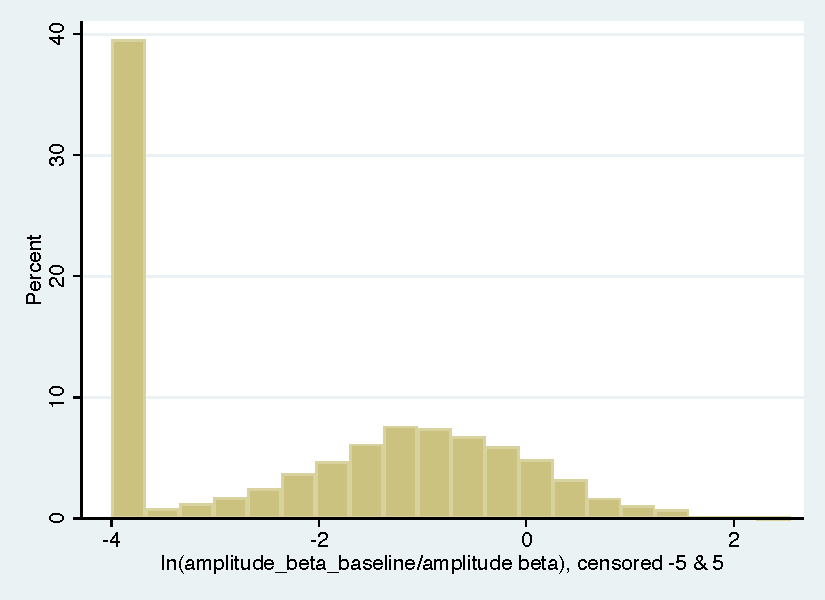
\includegraphics[height=4in]{accuracy_beta.pdf}
\end{center}
\end{figure}

Figure \ref{fig:accuracy_beta} In most cases, the log of the ratio is negative, implying a lower interval confidence of the $\beta$ estimate with our methodology. Our method undoubtedly yields more accurate estimations of the share of additive components, whatever the transport mode considered. We have checked that a similar conclusion applies on other years (they are not reported here for sake of brevity but they are available upon request).

\end{itemize}
\end{itemize}

All these elements drive us to maintain our original estimation as benchmark method in the revised version, and we deeply hope to convince you of the relevance of this choice. However, we also want to keep track of this alternative method as further robustness check. Fr this purpose, we have amended the online Appendix with a section devoted to the referee's method.\textbf{ XXX TO BE DONE XXX CHECK THIS SECTION EXISTS IN THE ONLINE APPENDIX XXX}

%\textbf{stop here}



\subsubsection{Concerns about endogeneity}

\textit{\textbf{The endogeneity problem}: quoting Footnote 14 of the paper, the authors
are estimating ti and ts(k) as coefficients on the industry or country
dummies times $1/\widetilde{p}_{ik}$. [...] Based on the productivity-sorting model in Melitz (2003) or the quality-sorting
model in Baldwin and Harrigan (2010),  $1/\widetilde{p}_{ik}$ is either positively
or negatively correlated with $\epsilon_{ik}$. So, the NNLS estimates are biased; and
the bias has nothing to with the casual versus accounting interpretation of
the estimates. Accordingly, the one-line justification the authors provide
to not address the endogeneity problem is far from convincing.}

Indeed, this is a very important point. The referee states that, based on theoretical insights by \citet{melitz} or \citet{baldwin_harrigan}, $1/\widetilde{p}_{ik}$ is correlated in one direction on another with residuals $\epsilon_{ik}$. In other words, more productive firms and/or firms selling high-quality products will charge higher prices, all other things equal – in our case, for a given country-product pair.

We obviously do not question this conceptual issue. However, it is worth noting that a good deal of the bias (actually, the part relating to the quality effect) is going to appear identically in the CIF (p) and the FAS ($\widetilde{p}_{ik}$) prices. Consequently, since our dependent variable is based on a ratio between the former and the latter, the (reverse causality) bias cancels out. That said, remains the possibility that bigger firms may impact transport costs, due to their ability of bargaining discounts for larger shipped volumes.

Following the referee's advice, we decided therefore to provide a full set of IV estimates to provide a clean assessment of the size of the potential bias. Section 4.3 in the revised version of the paper provides an overview of the results, while section B.4 in Appendix B provides a full presentation of the theoretical basis for the first-stage equation, as well as first-stage estimates. We follow earlier literature (see e.g. Caliendo and Parro, 2015, or Lashkaripour, 2017) by implementing a first-stage equation regressing $\widetilde{p}$ on custom duties coming based on tariffs at the product line, together with one-year lagged fas prices. First-stage estimates reported in section B.4 show that our main instrumental variable displays the right statistical properties, and that we can confidently re-inject the predictions arising from the first-stage equation for $\widetilde{p}_{ik}$ on the right-hand side of Equation 10 to produce a 2SLS-type of estimation. Figure 9 in the revised version of the paper reports our benchmark estimates by transport mode, together with their instrumented counterpart. In all cases, these estimates are very similar, when not identical. This supports that our benchmark estimates do not suffer any substantial biases arising from endogeneity concerns.

Not this check is performed both on our main dataset (SITC 5 digit), and also at the HS 10 level, to handle simultaneously the referee's concern about aggregation issues. In the latter case, second-stage estimates are not reported for the sake of space, but do not change anything to previous conclusion - they are very, very similar to their non-IV, least squares counterparts.


\subsubsection{The aggregation problem}

\textit{\textbf{The aggregation problem}: The original annual Census data reports
trade at the origin country-HS10 product-district level of aggregation,
whereas the authors are aggregating up the data even further to the origin
country-HS5 industry-year level. Such an aggregation comes with strong implicit assumptions and sacrifices a lot of useful variation in the data.
The authors are motivating the aggregation by stating that the problem
would become computationally expensive without it. But this reasoning
brings us back to my original point that the authors can use the Hummel's
Methodology to circumvent the computational burden.}

It is true that the original annual Census data reports trade at the origin country-HS 10 product-district level of aggregation. Our initial choice of retaining $s=3$ at the sectoral level, $k=5$ at the product level was driven by the use of Hummel's dataset available over 1974-2004 with $k=5$ the finest degree of aggregation. We yet agree with the referee that jumping from $k=10$ to $k=5$ digits at the product level is detrimental to our ability to exploit useful variation in the data. In line with the referee's comment, we now run the estimation by considering $k$ at the HS10 classification level, not 5. After checking with the US Bureau of Census, data is only available since 1989, now available to 2019. We have hence asked for all available data at the time of revision (1989-2009), and we now present the results considering $s=3$ and $k=10$. This however deprives us from being able to exploit the period 1974-1988 at the aggregation level. \textbf{Que faire pour la periode 1974-1989 XXX TO BE DISCUSSED XXX}. Furthermore, the computational burden mentioned by the referee is not attributable to the product classification level $k=5$ or 10) but rather to the degree of sectoral classification ($s=3$ or 4) as it conditions the number of fixed effects. This explains why we consider the $s=4$ digit- sectoral classification level only for some years. We thank the referee for pointing this ambiguity in our paper, which drove us to rewrite the associated paragraph in the revised version of the paper \textbf{see XXXX TO BE DONE ??? XXX}

% XXX JH: UNLESS I AM MISTAKING, THE SHOPPING LIST BELOW HAS BEEN IMPLEMENTED XXX TO BE CONFIRMED
%\subsubsection{To sum up: What remains to be done}

%\begin{enumerate}
%\item\label{bp:3} Re-run our benchmark method with $s=3$ and $k=10$ over available years and compare the results ($t,\tau,\beta$ with our benchmark ones ($s=3,k=5$). Hopefully does not change much so that we can keep up the period 1974-1988? Consider this as our new benchmark. Answer to the critique about the aggregation problem.
%\item\label{bp:1} After running the referee's 1 method with $s=3$, $k=$10, show tables or figures comparing 1) the number of observations / countries / sectors 3D by year / transport mode when we do our empirical strategy vs the referee's strategy; 2) comparison of the $\beta$ between the two methods; 3) comparison of the precision of the $\beta$ estimation. Answer to the critique about the estimation strategy.
%\item\label{bp:2} IV-First-stage equation on fas price at the $s=3$, $k=10$-digit level, for all years; then 2d-stage estimate of $t,\tau, \beta$ with our methodology; compare with our results obtained in the submitted version. Answer to the critique about the endogeneity bias.
%\end{enumerate}

\subsection{Critique 2: Calculation of Unit Prices}

\textit{My second critique concerns the way the authors are calculating the unit prices.
The Census data reports the quantity of goods per observation. So, the authors
can calculate the unit price as Value/Quantity, which is consistent with how
price is modeled in standard trade models. Instead, the authors calculate unit
price as Value/Weight. This used to be a common exercise in the past where
many data-sets did not report Quantity. But, given their data, there is no
justification for the authors to calculate the prices this way.}

\textit{Calculating the unit price as Value/Weight presents the authors
with an additional endogenity problem. To elaborate, let $\omega_{ik} = Weight/Quantity$
denote the unit weight of the goods in observation $ik$. Also let $\widehat{p}_{ik} = Value/Quantity$
(unlike what the authors assume) denote standard definition of price}. As a consequence, making the link with the fas price we consider in the paper: $\widetilde{p}_{ik} = \widehat{p}_{ik} / \omega_{ik}$.

\textit{This paper is essentially estimating the following equation}:

\begin{equation*}
\ln\left(\frac{p_{ik}}{\widetilde{p}_{ik}}-1 \right)= \ln \left(\tau_{i} \times \tau_{s(k)} -1 +\frac{t_{i} + t_{s(k)}}{\widehat{p}_{ik}/\omega_{ik}} \right) + \epsilon_{ik}
\end{equation*}

\textit{instead of estimating}:


\begin{equation*}
\ln\left(\frac{p_{ik}}{\widetilde{p}_{ik}}-1 \right)= \ln \left(\tau_{i} \times \tau_{s(k)}-1 +\frac{t_{i} + t_{s(k)}}{\widehat{p}_{ik}} \right) + \epsilon_{ik}
\end{equation*}

%\textbf{GD20200708 Pourquoi n’introduit-il pas $\widehat{p}$ à gauche ?}
\textit{There is evidence that (i) $\omega_{ik}$ varies significantly within narrowly-defined product
categories, and (ii) $\omega_{ik}$ is negatively correlated with transport costs. So the
way the authors are calculating unit prices and estimating the model creates a
new (but avoidable) source of endogeneity.}

% MEMO: DO NOT FORGET TO REPORT THE ARGUMENTATION BELOW IN THE MAIN TEXT XXX
\paragraph{Our answer:}
\noindent The referee definitely has a point here, in the sense that Census data do report the quantity of goods. In addition, referee's remarks echo recent findings by Lashkaripour (\emph{Journal of International Economics}, 2020): based on US data very similar to ours over the period 1995-2015, the paper highlights, among other results, the unit weight of imported goods is indeed substantially heterogeneous even within narrowly-defined product categories and the cost of transportation increases more rapidly with unit weight than the cost of production. Finally, Lashkaripour (2020) finds accounting for the heterogeneity in export unit weights provides evidence in favor of the iceberg cost assumption regarding transport costs.

We devoted a lot of thought to a potential switch from weight to quantity to get cleaner unit prices. However, the latter appears really uneasy in our context for several, non-trivial reasons:

\begin{enumerate}
\item The information on quantity is not mode-specific, which is incompatible with our empirical strategy of estimation transport costs conditional on the transport mode, similarly as in Hummels (2004). We could of course restrict observations to single-mode flows, but that would alter our sample in a non-trivial way, raising some potential selection biases.

\item Second, units are not available for many years over our period, especially in the 1970s and the 1980s \textbf{XXX GUILLAUME, TO BE CONFIRMED AND SUPPORTEDXXX}; this is particularly problematic considering that the time length is crucial for the assessment of transport costs long-run dynamics, which is one of the main objectives of the paper.

\item Time length is especially important considering that, in the 1970s, trade composition was significantly different from today, with more goods for which correlation between weight and quality is likely to be less obvious \textbf{XXX GUILLAUME: EXAMPLES XXX}. At a more fundamental level, one may argue that considering the unit price as value/weight is relevant in our setting where we seek to identify transport costs. For instance, it makes sense that the shipment costs of cars do depend not only on the quantity of cars exported, but on the weight it makes, which is related to the volume it takes in the plane or the vessel. \textbf{XXX GUILLAUME: Do we have evidence, even anecdotal, on this point?}

\end{enumerate}

These motives altogether highlight that it would be too costly and uncertain in our context to switch from weights to quantities to compute unit prices. That said, do we have reason to believe this measure of unit prices generate significant deviations from the one relying on quantities?

\citet{Lashkaripour_JIE2020} does provide important results related to ours. In particular, his result of transport costs close to be totally iceberg is quite different from our own findings of additive costs representing 20 to 40\% of total costs. The two stories are not necessarily incompatible, however. First, beyond a longer time span, our database is exhaustive (\textbf{XXX GUILLAUME: TO BE CONFIRMED)}, and encompasses all goods and industries, while \citet{Lashkaripour_JIE2020}) restricts to indivisible/discrete goods representing a bit more 56\% of US total imports of goods. In this regard, when comparing Tables 1 and 10 in \citet{Lashkaripour_JIE2020}, one can see that the share of multiplicative costs tends to decrease with the share of discrete goods.\footnote{Also, note that the share of multiplicative costs is derived from a formulation - Equation (3) in Lashkaripour (2021) - that may produce noisier estimates compared to ours, as we point in answer 2.1.ii to your Critique 1 above XXX \textbf{GUILLAUME : TO BE DISCUSSED AGAIN TOGETHER XXX}} It is therefore reasonable to think that the inclusion of all goods, like in our setting, would move the average share of multiplicative costs far from 100\%.

%\textbf{We make this point clear in Footnote XXX}


%\textbf{EN MEME TEMPS: Si on écarte de l'analyse les flux qui sont passés à la fois par bateau et par air, en ne gardant que les flux qui ont fait l'un ou l'autre, ne peut-on pas se dire que la quantité (pas mode-spécifique) a totalement voyage par vessel (si le flux indique qqch pour ves-val) ou par avion (s'il indique qqch pour air-val)? Et à ce moment là, on peut répondre ``vraiment'' à sa critique?} \textbf{GD20200708 Sauf que du coup, on change le sample. Il faudrait vérifier si c’est de beaucoup ou pas}


%\textbf{Je ne comprends pas bien le point (i)}. We thank the referee for pointing out this potential source of bias in our estimates. If we cannot follow the referee's advice be replacing weight by quantity for data availability reasons, we can address his/her concern regarding this as source of endogeneity bias by instrumenting the fas price. \textbf{il ne faudrait pas dans ce cas mettre de lagged prices, sinon on reintroduit du bruit. Non? Mais alors, on n'explique plus grand chose... }
%\textbf{GD20200708 Moi non plus je ne comprends pas très bien}

\subsection{Critique 3: Big Picture Implications}

\textit{My third critique concerns the lack of an exciting punchline. The fact that
composition effects have not countervailed the reduction in pure transport costs
(at least not as much as previously believed) is an interesting but minor observation.
Does this observation revise our understanding of say the gains from
trade? Does it shed new light on a puzzle many people are thinking about?
One crude suggestion is to see how the reduction in the industry-specific cost
terms is related to the industry-level trade elasticities. If the composition effects
favor low-elasticity industries, the findings in the paper may have first-order
implications for the gains from trade.
Another suggestion is to dig deeper into the relative rate at which additive
and multiplicative transport costs have declined over time. Since additive transport
costs favor rich (high-quality exporting) countries, the disproportionally
greater reduction in additive costs can perhaps explain the rise of low-income
exporter as documented by Hanson (2012, JEP).}

\paragraph{Our answer:}
\noindent We devoted a lot of thought to this point, which directly echoed a similar concern by the other referee. Taking stock of your suggestion, we decided to offer insights on the welfare implications of our results. In this regard,% the section 3.4 from the initial version has been moved to Appendix XXX TO BE DONE XXX of the paper,
the new section 5 ``The role of additive cost: Theoretical insights'' is devoted to a theory-based analysis of the alterations to welfare gains involved by the relative variations of additive and multiplicative transport costs over our period of analysis. \citet{melitz}, featuring additive trade costs. The inclusion of additive costs in a \citet{melitz} setting has already been performed in \citet{sorensen2014} and \citet{Irrazabal_2015}. However, \citet{sorensen2014} exclusively performs a theoretical analysis, without any quantitative exercise. In addition to a partial equilibrium extension of \citet{melitz}, \citet{Irrazabal_2015} do perform a quantitative simulation to assess the welfare variations induced by the presence of additive costs, but the latter is based on a calibration for transport costs restricted to 2004, based on the case of Nowrway. In contrast, our own exercise relies on a several decades time span for the US, allowing us to highlight the welfare alterations induced over time by the relative dynamics of additive and multiplicative costs, based on ``true'' values for the latter - remember that our methodology allows for the identification of both multiplicative and additive costs as a share of total costs, whereas additive costs in \citet{Irrazabal_2015} are expressed relatively to the (median) export price.

More precisely, we use some of the estimates underlying results reported in sections 2 and 3 concerning multiplicative and additive costs, more precisely those for the years 1974 and 2019. Based on the latter, we implement several comparative static exercises to investigate the different welfare consequences of alterations to multiplicative and additive costs. In addition, we also assess how the latter results are distorted by changes in sunk costs of exports, $f_{x}$. To that end, we adjust the share of exporting firms in the US: based on \citet{Lincoln_McCallum2018}, we set the latter to 35\% in 2019, versus 21\% in 1974.

Table 5 in section 5 in the revised version reports the results of these various comparative static exercises for Air and Vessel transport modes. Specifically, we report the change in total transport costs (expressed in percentage points, and based on the raw numbers reported in Table \ref{tab:calib_TC}), decomposed in its two dimensions (additive and ad-valorem); as well as the welfare change, both in absolute and in relative terms. For each transport mode, the first two columns report the results of reducing transport costs only, maintaining the same value of $f_x$ as in the initial equilibrium (Columns (A)-(B) for Air, (E)-(F) for Vessel), contrasting the case of only ad-valorem costs (Columns (A), (D)) and in presence of additive costs (Columns (B), (F)). Columns (C)-(D) for Air and (G)-(H) for Vessel report the results when both the variable transport costs and the fixed export costs are lower in the final steady state (2019) relative to the initial one (1974).

Qualitatively, the conclusions are identical for both transport modes, with two major insights. First, for a given decrease in transport costs,  welfare gains are around 50\% higher when the underlying framework allows for additive costs - which, in practice, concentrate the major part of transport costs decrease over the period. Second, the decrease in export sunk costs (i.e., increase in the share of exporting firms) proportionally amplifies the gains from decreasing costs, with again an additional premium coming from the decrease of additive costs. Quantitatively, welfare gains are more important for the Vessel mode, which is a natural consequence of a more substantial decrease in transport costs. More importantly, we see that the amplification effect coming from the decrease in $f_{x}$ is slightly lower for the specification including additive costs  in Vessel than in Air: a bit more than 40\% additional welfare gains for the former, versus 47\% gains for the latter. This reflects a slightly more balanced contribution from each component (additive and multiplicative) in the decrease of transport costs in Vessel compared to Air. This also emphasizes that the amplification effect of the decrease in sunk costs affects disproportionately the variations in additive costs.

Overall, these results appear to add a substantial contribution to the paper : we are able to provide a quantitative assessment of the welfare gains induced by the decrease in both types (additive and multiplicative) of costs over a 45 years period, and to highlight the respective part of each component in the determination of these gains. Note also that not only the inclusion of additive costs in the underlying framework generates big welfare differences, but also that the latter are probably a lower bound of the welfare variations induced by changes in additive \emph{trade} costs, larger than the sole transport costs.





%XXX is chosen to match the share of firms exporting in Norway (38 percent, Moxnes, 2010), while

%IMO : The data cover all Norwegian non-oil exporters in 2004 and originate from customs declarations.



%\textbf{Comments about that}

%\paragraph{Piste 1} Consider his/her first suggestion. What is the idea? First, the link between gains from trade and trade-elasticity. Am I correct in saying that gains from trade are higher when trade is about low-elasticity goods? The idea being, if national goods are low substitutes, then here are larger gains from trading them. So, if composition effects (trade shifts between sectors) favor low-elasticity sectors, then one might expect high gains from trade. Hummels: trade composition effects matter as they partially offset the reduction in pure transport costs for both air and vessel. Over time, tendency to trade goods more costly to export everything else equal. So, if the referee's assertion is right (trade composition effects favor low-elasticity sectors), then increasing gains from trade. But, we disagree with Hummel's findings (his way of measuring things is inappropriate) and find that trade composition effects do not matter much, at least for air (for vessel, the composition effects matter more, but by amplifying the reduction in transport costs, ie towards goods that are less costly to export). Meaning that gains from trade are purely due to reduction in transport costs at the sector, but not from switch towards low-elasticity sectors. Identify one source of gains from trade, not two.

%What to do with this? When composition effects do matter (ocean freight), do they favor low-elasticity industries? In which case, on top of the reduction in transport costs per se (which has welfare consequences as well), one might expect additional gains from these composition effects. When they don't, this mitigates the gains from trade that could be expected from the picture given by Hummels.

%\textbf{GD20200708 Hum... Je crois que je comprends le point dur referee et je suis d’accord avec lui. Le souci, c’est que de toutes les manières, je ne sais pas si cela favorise les high ou les low elasticity. Mais on pourrait voir.}

%\paragraph{Piste 2} What is at stake? Show that how $\beta$ = the relative share of additive costs has evolved over time. Good idea as this is really what differentiates us from Hummels, model a varying $\beta$ over time. Specifically, how methodology lets the $\beta$ vary over the three time-sector-partner country dimension. Show how $\beta$ varies over time everything else equal? Hopefully, goes in the referee's direction (decreases over time) with possibly a role in the understanding in the ``big picture'' of trade patterns?

%\paragraph{Piste 3} \textbf{GD20200708 On sait que les additive costs sont plus distorsifs que les multiplicative costs, puisqu’ils modifient les prix relatifs. Donc le fait qu’ils sont une partie croissante des costs signifie qu’on sur-estime l’augmentation des gains de welfare liés à la baisse des coûts de transport}

\newpage
\bibliographystyle{apalike2}
\bibliography{biblio}


\newpage

\appendix

% XXX JH: What do we do with the section below?

\section{Clarifying some technical points \label{app:technical_points}}


\subsection{A note on prices}

We have three prices: the (US) consumer price, say $p^{c}_{ik}$, the ``import'' or  cif price (at the entrance of the US) $p_{ik}$ and the fas price (at the export gate in the origin country) $\widetilde{p}_{ik}$, denoting $i$ the origin country, $k$ the product at the 8 or 5 digit level, and reasoning on a yearly basis, and $s(k)$ the 3-digit classification the product $k$ belongs to. Further, if we denote $\tau^d_{ik}$ the duty tax rate paid when the good crosses the US border, then we have:

\begin{eqnarray*}
&&p^c_{ik} = (1+\tau^d_{is(k)})p_{ik} \\
with && p_{ik}  = \tau_{is(k)} \widetilde{p}_{ik} +t_{is(k)}
\end{eqnarray*}


\subsection{Deriving the share of additive costs in total transport costs \label{app:interpret_beta}}


With $i$ the origin country, $k$ the product category at the HS6 level (and reasoning at the year- transport mode level), $p_{ik}$ the import (cif) price and $\tilde{p}_{ik}$ the export (fas) price, transport costs $f_{ik}\equiv \frac{p_{ik}- \tilde{p}_{ik}}{\tilde{p}_{ik}} $ are written in Hummel's terminology as:


\begin{equation}
f_{ik} = X_{is(k)}\tilde{p}_{ik}^{-\beta_{ik}} \label{eq:Hummels}
\end{equation}

It is trivial to show that:
$$\frac{\partial f_{ik}}{\partial \tilde{p}_{ik}} \frac{\tilde{p}_{ik}}{f_{ik}}= -\beta_{ik}$$

Then
\begin{itemize}
\item If $\beta_{ik} = 0$, then $p_{ik} = (1+X_{is(k)})\tilde{p}_{ik}$: Only ad-valorem transport costs
\item If $\beta_{ik} = 1$, then $p_{ik}=\tilde{p}_{ik}+X_{is(k)}$: Only additive costs
\end{itemize}

This suggests that, the closer $\beta_{ik}$ to 1, the more prevalent additive costs in total transport costs. Can $\beta_{ik}$ be related to the share of additive costs in total transport costs? The answer is positive. To show this clearly, start from:

\begin{eqnarray*}
f_{ik} &=& \frac{p_{ik}-\tilde{p_{ik}}}{\tilde{p}_{ik}}\\
\text{with}:&& p_{ik} = \tau_{is(k)}\tilde{p}_{ik} + t_{is(k)} \\
\end{eqnarray*}

assuming that transport costs decompose in two components, additive transport costs $t_{is(k)}$ and multiplicative costs (ad-valorem) $\tau_{is(k)}$, supposed to be identical in the product-dimension for any $k$ product within the 3-digit classification $s$ it belongs to.

This gives:

$$f_{ik} = \frac{(\tau_{is(k)}-1)\tilde{p}_{ik}+t_{is(k)}}{\tilde{p}_{ik}}$$

From this, we have

\begin{eqnarray*}
\frac{\partial f_{ik}}{\partial \tilde{p}_{ik}} &=& \frac{(\tau_{is(k)}-1)\tilde{p}_{ik} - ((\tau_{is(k)}-1)\tilde{p}_{ik} +t_{is(k)})}{\tilde{p}_{ik}^2} \\
&=& \frac{-t_{is(k)}}{\tilde{p}_{ik}^2}
\end{eqnarray*}

Hence
\begin{eqnarray*}
\frac{\partial f_{ik}}{\partial \tilde{p}_{ik}} \frac{\tilde{p}_{ik}}{f_{ik}}&=& \frac{-t_{is(k)}}{(\tau_{is(k)}-1)\tilde{p}_{ik} +t_{is(k)}}\\
&=& \frac{-\frac{t_{is(k)}}{\tilde{p}_{ik}}}{\tau_{is(k)}-1 +\frac{t_{ik}}{\tilde{p}_{ik}}}
\end{eqnarray*}

This shows that $\beta_{ik}$ can be interpreted as the share of additive costs in total transport costs:

$$\beta_{ik} = \frac{\frac{t_{is(k)}}{\tilde{p}_{ik}}}{\tau_{is(k)}-1 + \frac{t_{is(k)}}{\tilde{p}_{is(k)}}} $$


\subsection{Share vs level}

Starting from the above reasoning, the referee proposes to estimate the elasticity of transport costs with respect to the unit price, equivalently the share of additive costs in total costs. Specifically, the referee suggests to estimate for each industry-country the following regression:

$$\ln f_{ikd}= \beta_{is(k)} \ln \widetilde{p}_{ikd} + \text{Controls}_{ikd} +\epsilon_{ikd}$$

The question is then, how to recover the levels of additive / multiplicative transports costs $t_{is(k)}$ and $\tau_{is(k)}$. Denoting $\widehat{\beta}_{is(k)}$ the estimated $\beta$ from the referee's method for a given sector-country $i,s(k)$, one can solve the following two-equation system:

\begin{eqnarray}
p_{ik} &=& \tau_{is(k)}\widetilde{p}_{ik} +t_{is(k)} \label{eq:system1}\\
\frac{t_{is(k)}}{(\tau_{is(k)}-1)\widetilde{p}_{ik}} &=& \widehat{\beta}_{is(k)}  \label{eq:system2}
\end{eqnarray}

\noindent with $p_{ik}$ and $\widetilde{p}_{ik}$ the cif and fas prices observed in our dataset (conditional on a given year-transport mode). With 2 equations and 2 endogenous variables, the system might be solved. Specifically, with $\widehat{\beta}$ being estimated at the \textit{sector} $s$- country $i$ level, and $\widetilde{p}_{ik}$ at the \textit{product} $k$-country level, this implies that $t$ and $\tau$ are product-country $i,k$ specific (not sector-country $s,k$ specific). \textbf{from this point of view, this is a finer characterization of transport costs, so better from this point of view...}

To show this properly, start from Equation (\ref{eq:system2}) to express additive costs according to:
$$t_{ik} = \frac{ \widehat{\beta}_{is(k)}}{1- \widehat{\beta}_{is(k)}} \left[\tau_{is(k)}-1\right]\widetilde{p}_{ik} $$

With $\widetilde{p}_{ik} $ being product-country specific, $t_{ik}$ is necessarily product-country specific ($i,k$, not $i,s(k)$). Plugging this into Equation (\ref{eq:system1}):

$$p_{ik} = \tau_{is(k)} \widetilde{p}_{ik} + \frac{ \widehat{\beta}_{is(k)}}{1- \widehat{\beta}_{is(k)}} \left[\tau_{is(k)}-1\right]\widetilde{p}_{ik} $$

Solving for $\tau$, one finally obtains the solutions for the ad-valorem and additive transport costs components:

\begin{eqnarray}
\tau_{ik} & =& (1-\widehat{\beta}_{is(k)}) \frac{p_{ik}}{\widetilde{p}_{ik} } + \widehat{\beta}_{is(k)} \label{eq:tau_method_ref1}\\
t_ik &=& \frac{ \widehat{\beta}_{is(k)}}{1- \widehat{\beta}_{is(k)}} \left[\tau_{is(k)}-1\right]\widetilde{p}_{ik} \label{eq:t_method_ref1}
\end{eqnarray}


Two points can be made. First, we can check that if $\widehat{\beta}_{is(k)}=0$, then $p_{ik} = \tau_{ik} \widetilde{p}_{ik}$ (Equation \ref{eq:tau_method_ref1}) and $t_{ik} = 0$ (Equation \ref{eq:t_method_ref2}), all transport costs are ad-valorem. Conversely, if $\widehat{\beta}_{is(k)}=1$, then $p_{ik} = \widetilde{p}_{ik} + t_{ik} $ (Equation \ref{eq:tau_method_ref2}) and $\tau_{ik} = 0$ (Equation \ref{eq:t_method_ref1}). Second, and most importantly, the method allows to recover the levels of both transport costs components at the product-country level $i,k$, even though the share of additive costs in total costs is estimated at the sector-country level.



\end{document}


\section{More details on the instrumentation strategy}

\subsection{Specification of the first stage equation}


The question we deal with, is the functional form of the first stage equation, where we instrument the fas price with duties as suggested by Referee 1. The idea is that firms might react to changes in duty tax rates which have nothing to do with transport costs changes. In this respect, considering the predicted part of the fas price related to tax duty is likely to solve potential endogeneity biases.

Denoting $i$ the origin country, $k$ the product at the 5 digit level, and reasoning on a yearly basis, if we assume that the fas price $\widetilde{p}_{ik}$ decomposes in two components, say $\bar{p}_{ik}$ the ``firm-specific'' price (related to its cost and pricing strategy) and $\tau^d_{ik}$ the tax duty (out of the firm's hands) according to :

\begin{equation}
\widetilde{p}_{ikt} = (1+\tau^d_{is(k)t})^\alpha \left(\bar{p}_{ikt}\right)^\beta \label{eq:link_fas_duty}
\end{equation}

\noindent with $s(k)$ the 3-digit classification as a function of the 5-digit product classification.

\subsubsection{First-stage equation in first difference \label{ssec:first_diff}}

One option to specify the functional form of the first stage is to take the total differential around some reference point at time $t-1$, with $\Delta $ the difference operator ($\Delta\widetilde{p}_{ikt} = \widetilde{p}_{ikt} - \widetilde{p}_{ikt-1}$ and so on):
\begin{eqnarray*}
&&\Delta \widetilde{p}_{ikt} = \beta \bar{p}_{ikt-1}^{\beta-1}(1+\tau^d_{is(k)t-1})\Delta \bar{p}_{ikt} + \alpha \bar{p}^\beta_{ikt-1} (1+\tau^d_{ikt-1})^{\alpha-1}\Delta \tau^d_{is(k)t}  \\
\Leftrightarrow &&\frac{\Delta \widetilde{p}_{ikt}}{\widetilde{p}_{ikt-1}} = \beta \frac{\Delta \bar{p}_{ikt}}{\widetilde{p}_{ikt-1}} \frac{(1+\tau^d_{is(k)t-1})^\alpha \bar{p}_{ikt-1}^\beta}{\bar{p}^\beta_{ikt-1}(1+\tau^d_{is(k)t-1})^\alpha} +\alpha \frac{\Delta \tau^d_{is(k)t-1}}{1+\tau_{is(k)t-1}^d}\frac{(1+\tau^d_{is(k)t-1})^\alpha \bar{p}_{ikt-1}^\beta}{\bar{p}^\beta_{ikt-1}(1+\tau^d_{is(k)t-1})^\alpha} \end{eqnarray*}

leading to:
\begin{equation}
\frac{\Delta \widetilde{p}_{ikt}}{\widetilde{p}_{ikt-1}} =  \beta \frac{\Delta \bar{p}_{ikt}}{\bar{p}_{ikt-1}} +\alpha\frac{\Delta \tau^d_{is(k)t}}{1+\tau_{ikt-1}^d} \label{eq:firststage_Deltalog}
\end{equation}

The intuition behind the Referee 1's endogeneity concerns, is that we need to eliminate from the fas price, any endogenous component that might me related to transport costs. To do so, the referee suggests that we instrument the export price by tariff rates. Put it in plain words, this suggests to run the first-stage regression based on Equation (\ref{eq:firststage_Deltalog}) according to:

$$\frac{\Delta \widetilde{p}_{ikt}}{\widetilde{p}_{ikt-1}} = \alpha \frac{\Delta \tau^d_{is(k)t}}{1+\tau_{is(k)t-1}^d} + \gamma_{i} +\gamma_{k}+\epsilon_{ik}$$

Or equivalently, taking logs:
$$\Delta \log \widetilde{p}_{ikt}= \alpha\frac{\Delta \tau^d_{is(k)t}}{1+\tau_{is(k)t-1}^d} +\gamma_{i} +\gamma_{k}+\epsilon_{ikt}$$


\noindent with the LHS being the growth rate of the fas price (between $t$ and $t-1$), the first term in the RHS the change in duty tax rates, the second and third terms fixed effects to capture changes in the ``firm-specific price'' $\bar{p}_{ik}$, $\epsilon_{ik}$ being the residual. Notice though that the structure of fixed effects should remain consistent between the first and the second stages. This implies to rather consider the following functional form of the first-stage equation:

\begin{equation}
\Delta \log \widetilde{p}_{ikt} = \alpha\frac{\Delta \tau^d_{is(k)t}}{1+\tau_{is(k)t-1}^d} +\gamma_{i} +\gamma_{s}+\epsilon_{ikt} \label{eq:firststage_Deltalog}
\end{equation}

If this reasoning is correct,
\begin{itemize}
\item we should take as predicted value only the predicted price without the fixed effects:
$$\left(\frac{\Delta \widetilde{p}_{ikt}}{\widetilde{p}_{ikt-1}}\right)^{IV} = \widehat{\alpha}\frac{\Delta \tau^d_{is(k)t}}{1+\tau_{is(k)t-1}^d} $$
\item and we should expect a value of the coefficient $\widehat{\alpha}$ between $\Delta \log \widetilde{p}_{ikt}$ and $\frac{\Delta \tau^d_{is(k)t}}{1+\tau_{is(k)t-1}^d} $ between $-1$ and $0$, depending on the degree of ``pricing-to-market'' of firms.
    \begin{itemize}
    \item[-] $\alpha = 0$ corresponds to the case where the firm does not adjust its fas price to the change in tax duty, that would cancel out the influence of the tax duty change on the price paid by the US consumers; this rather corresponds to small firms which do not have enough market power to manipulate their prices following changes in international competition;
    \item[-] $\alpha <0$ corresponds to the degree of``pricing-to-market'' as the firm offsets the impact of the tax change of the price paid by the final consumer by adjusting her producer price in the opposite direction of the tax change,
    \item[-] with $\alpha = -1$ being the extreme case of ``full PTM'' where the firm fully compensates the tax duty change. As shown by Berman, Martin, Mayer (REStats 2012), this is more likely larger firms.
    \end{itemize}
\end{itemize}

Once this is done, we can rebuild the instrumented fas price in level (at time $t$):

\begin{eqnarray*}
\widetilde{p}^{IV}_{ikt} = \widetilde{p}_{ikt-1}\left[1 + \left(\frac{\Delta \widetilde{p}_{ikt}}{\widetilde{p}_{ikt-1}}\right)^{IV}\right]
\end{eqnarray*}

with $\widehat{\widetilde{p}}_{ikt}$ the instrumented fas price at time $t$, for product $k$ from country $i$; $\widetilde{p}_{ikt-1}$ the observed lagged fas price for the same $i,k$ couple; and $ \left(\frac{\Delta \widetilde{p}_{ikt}}{\widetilde{p}_{ikt-1}}\right)^{IV}$ the predicted growth rate of the fas price based on duty changes.

\subsection{First-stage equation in level}

Alternatively, one can run the first-stage equation in log level, consistently with the second-stage log-level specification. Further, in accordance with the referee's suggestion, this also implies including the lagged price as instrument. Starting from Equation (\ref{eq:firststage_Deltalog}), we thus run as first-stage specification:


\begin{equation}
\log \widetilde{p}_{ikt} = \alpha\frac{\Delta \tau^d_{is(k)t}}{1+\tau_{is(k)t-1}^d} + \beta \log\widetilde{p}_{ikt-1}  +\gamma_{i} +\gamma_{s}+\epsilon_{ikt} \label{eq:firststage_log}
\end{equation}

Consistently with the cross-section analysis adopted by now, the first-stage equation is estimated on a yearly basis (and by transport mode). We then build the instrumented fas price

\begin{eqnarray*}
&&\log \widetilde{p}_{ikt}^{IV} = \widehat{\alpha}\frac{\Delta \tau^d_{is(k)t}}{1+\tau_{is(k)t-1}^d} + \widehat{\beta}\log\widetilde{p}_{ikt-1} \\
\rightarrow &&\widetilde{p}_{ikt}^{IV}  = \exp^{\log \widetilde{p}_{ikt}^{IV}}
\end{eqnarray*}
